\documentclass[12pt,letterpaper]{article}

\marginparsep 0pt
\textwidth 6in
\topmargin 0pt
\headsep .5in
\textheight 8.7in
\voffset = 0pt
\hoffset = 0pt
\marginparwidth = 0pt
\oddsidemargin = 0pt

\usepackage[utf8]{inputenc}
\usepackage[spanish]{babel}
\usepackage{graphicx}
\usepackage{graphics}
\usepackage[dvips]{epsfig}
\usepackage[dvips]{graphicx}
\usepackage{rotating}
\usepackage{multirow}
\usepackage{array}
\usepackage{longtable}
\usepackage[]{fontenc}
\usepackage[nottoc,notlot,notlof]{tocbibind}


\addto\captionsspanish{
\def\listtablename{\'Indice de tablas}
\def\tablename{Tabla}
}

\begin{document}
\begin{center}
\begin{figure}[ht]
\begin{center}

\includegraphics[scale=0.5]{logoUV.png}
\end{center}
\end{figure}
\thispagestyle{empty}

UNIVERSIDAD DE VALPARAÍSO \\
Facultad de Ingeniería \\
Escuela de Ingenier\'ia Civil Inform\'atica \\
Ingenier\'ia Civil en Inform\'atica\\
\vspace{1cm}
\Large
\textbf{Sistema de Minería de Datos para apoyar la toma de decisiones de profesionales de PPF AITUE}\\ 
\large 
Propuesta de Trabajo de T\'itulo \\
Marcelo Esteban Verdugo Reyes \\
\normalsize
\emph{marcelo.verdugor@alumnos.uv.cl} \\
\today \\
\vspace{1cm}
Profesor Gu\'ia:
Eliana Paz Providel Godoy
\end{center}



\begin{abstract}


En Chile existen diferentes familias que se encuentran en situaciones de riesgo, el cual repercute, ocasionalmente en vulneraciones de los derechos de los niños, niñas y adolescentes (NNA). Existen distintas instituciones para la protección de los integrantes de las familias dentro de estas se encuentran las corporaciones que buscan intervenir en ellas con el fin de brindar apoyo en las tareas de crianza y desarrollo personal de los NNA. 
En estas corporaciones los especialistas capacitados utilizan diferentes herramientas para analizar situaciones de riesgo en la cual se ven insertas estas familias, donde la experiencia en la toma de decisiones juega un rol fundamental.\\ 
Estas corporaciones por lo general no disponen de herramientas que utilicen Tecnologías de Informaci\'on y Comunicaci\'on (TIC) por lo cual en este Trabajo de T\'itulo se busca apoyar a los especialistas con herramientas TIC, para as\'i agilizar sus procesos y tambi\'en ser de ayuda a la hora de tomar decisiones.



\end{abstract}



\newpage

\tableofcontents
\newpage

\listoftables
\listoffigures
\newpage



\section{Introducci\'on}
\label{intr}

Uno de los derechos fundamentales de los NNA es que sus necesidades sean satisfechas para desarrollarse y alcanzar la madurez. 
Esta tarea, principalmente recae en los padres y cuidadores, pero además de ellos, también se ven involucrados el conjunto de la sociedad en la que se encuentran los NNA. Por lo cual es necesario que cada adulto, cada comunidad y cada Estado disponga de los cuidados, la protección y la educación que estos necesitan para llegar a la adolescencia y luego a la vida adulta, de una forma sana, constructiva y feliz \cite{REF1}.

Está demostrado \cite{REF2} que los trastornos del desarrollo, comportamientos agresivos y violentos, así como otras manifestaciones negativas de los NNA, tienen una estricta relación cuando estos son víctimas y testigo de violencia en el ámbito familiar. Por lo cual es necesario prevenir los malos tratos infantiles para evitar desencadenar estas conductas negativas. 
En la región de Valparaíso existen varias poblaciones con altos porcentajes de pobreza. Una de ellas es Forestal, en donde se puede observar que los menores de edad se caracterizan por ser víctimas de maltrato y negligencia, agresiones verbales, físicas y/o descalificaciones de mayor o menor gravedad; son testigos de violencia intrafamiliar. Entre los niños y niñas de edad preadolescente se observa bajos niveles de autoestima y percepción de logros; recurrentes problemas conductuales, malos tratos a nivel familiar y de pares, ausentismo y riesgo de deserción escolar y bajo rendimiento académico. Entre la población adolescente es posible observar conducta sexual precoz y/o de riesgo, conflictos delictuales, uso de alcohol y/o drogas, embarazo precoz, deserción escolar, microtráfico,  falta de proyectos de vida \cite{REF3}. 
Por estos motivos nacen diferentes proyectos, uno de ellos es el Programas de Prevención Focalizada PPF AITUE, el cual tiene por objetivo que los niños, niñas y adolescentes fortalezcan sus recursos personales, autoestima, autoimagen y habilidades sociales. Junto con ello, que los adultos responsables cuenten con las herramientas y oportunidades para el ejercicio de una parentalidad positiva y que las familias cuenten con apoyos para favorecer la crianza y el desarrollo de los niños, niñas y adolescentes. 
Este programa se encuentra ubicado en la población de Forestal Alto en Viña del Mar. 
 
El Programa de Prevención Focalizada PPF AITUE utiliza diferentes herramientas al momento de trabajar con las familias y los NNA.
En un principio se realiza un análisis de la situación actual familiar. Para esto el profesional se dirige al hogar de los menores con el fin de poder observar las condiciones en la que él y su familia conviven, además realiza entrevistas para que posteriormente con la información obtenida, el profesional logre formar un juicio del funcionamiento familiar actual.
Posteriormente se utiliza una herramienta llamada NCFAS que es una apreciación del profesional con respecto a la familia.
 

\section{Definición del Problema}
\label{def}

\subsection{Problema}
Actualmente los profesionales del PPF AITUE utilizan herramientas de evaluación, las cuales capturan la estructura ecológica del funcionamiento familiar \cite
La principal herramienta que utilizan estos profesionales es la herramienta NCFAS (North Carolina Family Assessment Scale). Esta escala de evaluación está integrada de una serie de indicadores de gran relevancia las cuales se agrupan en diferentes dimensiones. Para llenar esta escala el profesional realiza visitas domiciliarias y cuestionarios, donde dicha información permite al profesional formarse un jucio sobre las características del funcionamiento familiar actual. Posteriormente la herramienta permite ordenar esta información y además exige la asignación de puntajes a las diferentes dimensiones que cubre. 
Este formulario (en papel) es llenado manualmente por el profesional lo que permite obtener un puntaje para cada dimensión evaluada, esta puntuación es analizada para ver si es necesario intervenir o no en la familia evaluada, con el fin de prevenir maltratos infantiles y negligencia parental.
De acuerdo a lo anterior, se detectan los siguientes problemas:

\begin{itemize}
\item Falta de una aplicación de escritorio que automatice el proceso de apreciación familiar de los profesionales del PPF AITUE
\item Falta de disposición de información digital de las apreciaciones familiares
\item Falta de información útil y no trivial para apoyar la toma de decisiones del profesional  
\end{itemize}

\subsection{Soluci\'on Propuesta}

Para dar solución a este problema se propone crear una aplicación de escritorio que permitirá al profesional del PPF AITUE automatizar el proceso de apreciación familiar que realiza actualmente con la herramienta NCFAS. Esta aplicación, además, dispondrá de diferentes módulos (estadística descriptiva y minería de datos), los cuales, entregarán al profesional información útil y no trivial para apoyarlo en la toma de desiciones con respecto a la prevención de maltratos infantiles y la negligencia parental. 



\subsection{Importancia del Trabajo}
Con el apoyo de esta aplicación el profesional, al realizar una nueva apreciación familiar podrá:
\begin{itemize}
\item Realizar el proceso de manera más eficiente
\item Encontrar información útil y no trivial para obtener apoyo a la hora de tomar desiciones, lo cual permitirá realizar un mejor preoceso de prevención de maltratos y negligencia parental 
\item \textit{Aumentar la cantidad de familias tratadas en el PPF AITUE}  
\end{itemize}



\section{Objetivos}
\label{obj}

\subsection{Objetivos generales}
El objetivo de este trabajo de título es desarrollar una aplicación que automatice la herramienta de apreciación NCFAS y que además, proporcione información útil y no trivial cuando un profesional del PPF AITUE realice una apreciacion familiar. 


\subsection{Objetivos espec\'ificos}

Para cumplir con el objetivo general es necesario cumplir los siguientes objetivos específicos:
\begin{itemize}

\item Realizar simulación de datos.

\item Analizar y comparar diferentes técnicas de minería de datos.
\item	Encontrar patrones dentro de los descriptores de la herramienta NCFAS, utilizando Minería de Datos. 
\item	Detección y predicción para la toma de decisiones basada en la simulación de datos. 
\item	Implementar las técnicas de Minería de Datos seleccionada. 
\item	Generar reportes según la técnica seleccionada. 

\end{itemize}

\newpage
\section{Metodolog\'ia}
\label{metod}

Para cumplir con los objetivos propuestos anteriormente, se realizará una metodología de trabajo del tipo cascada Incremental. 
Como se muestra en la Figura 1, esta metodología combina la metodología incremental la cual se lleva a cabo hasta la etapa de “Diseño”. Luego en la etapa de “Desarrollo de la primera iteración del Sistema” se da comienzo a una metodología del tipo incremental, la cual perdura hasta la etapa de “Validación del Sistema” donde luego se procede a retomar la metodología incremental.
En la Tabla 1 se explica cada una de las etapas que se muestran en la Figura 1.
%
\begin{figure}[htb]
\label{Figura 1}
\begin{center}
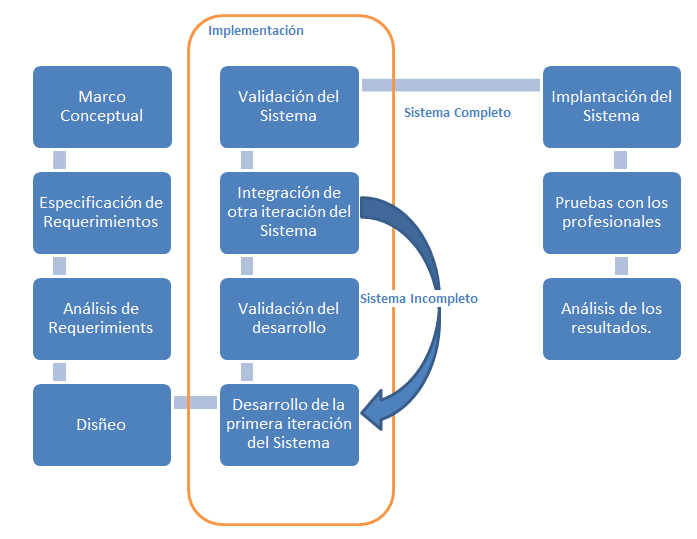
\includegraphics[scale=0.7]{metodologiaMV.png}
\end{center}
\caption{Metodolog\'ia de desarrollo del trabajo de t\'itulo.}
\end{figure}
%
\newpage
\clearpage

 

\begin{table}[hbt]
\begin{tabular}{| p{4.5cm} | p{4.5cm} | p{4.5cm} |}
\hline
\multicolumn{3}{|c|}{\textbf{\textit{Descripci\'on etapas metodología de trabajo}}} \\ \hline
\textit{\textbf{Etapas}} & 
\textit{\textbf{Descripción}} &  
\textit{\textbf{Productos}}
\\ \hline 
{Marco Conceptual} & 
{Se realiza una búsqueda bibliográfica acerca de aplicaciones que se hayan creado que utilicen los datos de la herramienta NCFAS.} & 
{Documento estado del arte.} 
\\ \hline
{Análisis y especificación de requerimientos.} & 
{Se recopilan y especifican los requerimientos necesarios para la creación de la aplicación.} & 
{Documento de Análisis y especificación de requerimientos.} 
\\ \hline
{Diseño} & 
{Diseño de la arquitectura del software, Diseño lógico de la aplicación, Diseño de pruebas, Diseño de datos, Diseño de interfaz de usuario.} & 
{Diagrama de arquitectura del sistema, diagrama de interacción, diagrama de clases, modelo interno lógico, esquemas de navegación, diseño de plan de testing, diseño de pruebas con alumnos.}
\\ \hline
{Desarrollo de la primera iteraci\'on del sistema.} & 
{Se desarrolla un sistema de escritorio, el cual se llevará a cabo mediante tres iteraciones. } & 
{Módulo de trabajo con NCFAS,  módulo de minería de datos y de estadística descriptiva.} 
\\ \hline
{Validaci\'on del desarrollo} & 
{Se aplica testing unitario a cada iteración implementada.} & 
{Resultado de testing y códigos corregidos.} 
\\ \hline
{Integración de otra iteración del sistema.} & 
{Se integra el incremento testeado y aprobado a la aplicación.} &
{Sistema anterior más una nueva iteración integrada.}
\\ \hline

\end{tabular} 
\label{Tabla 1}
 \end{table}

\newpage
\clearpage


%
\begin{table}[htf]
\begin{tabular}{| p{4.5cm} | p{4.5cm} | p{4.5cm} |}
\hline
\multicolumn{3}{|c|}{\textbf{\textit{Descripci\'on etapas metodología de trabajo}}} \\ \hline
\textit{\textbf{Etapas}} & 
\textit{\textbf{Descripci\'on}} & 
\textit{\textbf{Productos}}
\\ \hline
{Validación del sistema.} & 
{Por medio de testing de aceptación, se prueba y acepta el sistema completo.} & 
{Resultado de testing y códigos corregidos.} 
\\ \hline
{Implantación.} & 
{La aplicación es instalada y se encuentra lista para ser utilizada por los profesionales. Además se desarrolla una capacitación para los profesionales que necesiten utilizar la aplicación.} & 
{Instalación de la aplicación funcional.}  
\\ \hline
{Ejecución de pruebas con profesionales.} & 
{Se seleccionan profesionales del PPF AITUE y se realizan pruebas para la recopilación de nuevos datos de ingreso y egreso de familias.} &
{Nuevos datos de las pruebas realizadas.} 
\\ \hline
{Análisis de resultados. } & 
{Mediante minería de datos, se analizan los nuevos datos para observar patrones en el ingreso de los NNA al sistema.} & 
{Informe de los resultados de pruebas.} 
\\ \hline

\end{tabular}
\caption{Descripci\'on Metodolog\'ia.}
\end{table}

\newpage
\clearpage
%
\section{Planificaci\'on}
\label{plan}

El plan de desarrollo para lograr los objetivos planteados se describe en la \ref{Tabla 2}.

\begin{table}[htf]
\label{Tabla 2}
\begin{tabular}{| l | p{6cm} | l | l | l |}
\hline

\small{\textbf{ID}} & 
\small{\textbf{Etapas}} & 
\small{\textbf{Inicio}} & 
\small{\textbf{Fin}} & 
\small{\textbf{Antecesor}} \\ \hline

\textbf{\small 1.0.0} & 
\textbf{\small Marco Conceptual} & 
\textbf{\small 18/03/2015} &  
\textbf{\small 18/03/2015} & 
\textbf{\small -----} \\ \hline

\small 1.1.0 & 
\small - Búsqueda de material bibliográfico  & 
\small 18/03/2015 &  
\small 18/03/2015 & 
\small ----- \\ \hline

\small 1.2.0 & 
\small - Documentación & 
\small 18/03/2015 &  
\small 18/03/2015 & 
\small 1.1.0 \\ \hline

\textbf{\small 2.0.0} & 
\textbf{\small Especificación de Requerimientos} & 
\textbf{\small 18/03/2015} &  
\textbf{\small 18/03/2015} & 
\textbf{\small 1.0.0} \\ \hline

\small 2.1.0 & 
\small - Especificación de requerimientos funcionales  & 
\small 18/03/2015 &  
\small 18/03/2015 & 
\small 1.0.0 \\ \hline

\small 2.2.0 & 
\small - Especificación de no funcionales  & 
\small 18/03/2015 &  
\small 18/03/2015 & 
\small 1.0.0 \\ \hline

\small 2.3.0 & 
\small - Documentación & 
\small 18/03/2015 &  
\small 18/03/2015 & 
\small 2.1.0 - 2.2.0 \\ \hline

\textbf{\small 3.0.0} & 
\textbf{\small Análisis de Requerimientos} & 
\textbf{\small 18/03/2015} &  
\textbf{\small 18/03/2015} & 
\textbf{\small 1.0.0} \\ \hline

\small 3.1.0 & 
\small - Diagramas de Casos de Uso & 
\small 18/03/2015 &  
\small 18/03/2015 & 
\small 1.0.0 \\ \hline

\small 3.2.0 & 
\small - Modelo de entidad relación & 
\small 18/03/2015 &  
\small 18/03/2015 & 
\small 1.0.0 \\ \hline

\small 3.3.0 & 
\small - Documentación & 
\small 18/03/2015 &  
\small 18/03/2015 & 
\small 1.0.0 \\ \hline

\textbf{\small 4.0.0} & 
\textbf{\small Diseño} & 
\textbf{\small 18/03/2015} &  
\textbf{\small 18/03/2015} & 
\textbf{\small 1.0.0} \\ \hline

\small 4.1.0 & 
\small - Diagrama de Arquitectura & 
\small 18/03/2015 &  
\small 18/03/2015 & 
\small 1.0.0 \\ \hline

\small 4.2.0 & 
\small - Diagramas de navegación e interacción  & 
\small 18/03/2015 &  
\small 18/03/2015 & 
\small 1.0.0 \\ \hline

\small 4.3.0 & 
\small - Diagrama de clases & 
\small 18/03/2015 &  
\small 18/03/2015 & 
\small 1.0.0 \\ \hline

\small 4.4.0 & 
\small - Modelo intern lógico & 
\small 18/03/2015 &  
\small 18/03/2015 & 
\small 1.0.0 \\ \hline

\small 4.5.0 & 
\small - Diseño plan de Testing & 
\small 18/03/2015 &  
\small 18/03/2015 & 
\small 1.0.0 \\ \hline

\small 4.6.0 & 
\small - Diseño plan de pruebas con usuarios & 
\small 18/03/2015 &  
\small 18/03/2015 & 
\small 1.0.0 \\ \hline

\small 4.8.0 & 
\small - Documentación & 
\small 18/03/2015 &  
\small 18/03/2015 & 
\small 1.0.0 \\ \hline


\hline
\end{tabular}
\caption{Planificación desde Marco Conceptual hasta Diseño.}
\end{table}

\newpage
\clearpage

\begin{table}[htf]
\begin{tabular}{| l | p{6cm} | l | l | l |}
\hline
		
\small{\textbf{ID}} & 
\small{\textbf{Etapas}} & 
\small{\textbf{Inicio}} & 
\small{\textbf{Fin}} & 
\small{\textbf{Antecesor}} \\ \hline

\textbf{\small 5.0.0} & 
\textbf{\small Implementación} & 
\textbf{\small 18/03/2015} &  
\textbf{\small 18/03/2015} & 
\textbf{\small 1.0.0} \\ \hline

\small 5.1.0 & 
\small - Módulo ingreso de una nueva apreciación familiar & 
\small 18/03/2015 &  
\small 18/03/2015 & 
\small 1.0.0 \\ \hline

\small 5.1.1 & 
\small - Implementación & 
\small 18/03/2015 &  
\small 18/03/2015 & 
\small 1.0.0 \\ \hline

\small 5.1.2 & 
\small - Testing con usuarios & 
\small 18/03/2015 &  
\small 18/03/2015 & 
\small 1.0.0 \\ \hline

\small 5.1.3 & 
\small - Documentación & 
\small 18/03/2015 &  
\small 18/03/2015 & 
\small 1.0.0 \\ \hline

\small 5.2.0 &
\small - Módulo de estadística descriptiva & 
\small 18/03/2015 &  
\small 18/03/2015 & 
\small 1.0.0 \\ \hline

\small 5.2.1 & 
\small - Implementación & 
\small 18/03/2015 &  
\small 18/03/2015 & 
\small 1.0.0 \\ \hline

\small 5.2.2 & 
\small - Testing con usuarios & 
\small 18/03/2015 &  
\small 18/03/2015 & 
\small 1.0.0 \\ \hline

\small 5.2.3 & 
\small - Documentación & 
\small 18/03/2015 &  
\small 18/03/2015 & 
\small 1.0.0 \\ \hline

\small 5.3.0 &
\small - Módulo de Minería de Datos & 
\small 18/03/2015 &  
\small 18/03/2015 & 
\small 1.0.0 \\ \hline

\small 5.3.1 & 
\small - Implementación & 
\small 18/03/2015 &  
\small 18/03/2015 & 
\small 1.0.0 \\ \hline

\small 5.3.2 & 
\small - Testing con Usuarios & 
\small 18/03/2015 &  
\small 18/03/2015 & 
\small 1.0.0 \\ \hline

\small 5.3.3 & 
\small - Documentación & 
\small 18/03/2015 &  
\small 18/03/2015 & 
\small 1.0.0 \\ \hline

\textbf{\small 6.0.0} & 
\textbf{\small Validación del sistema} & 
\textbf{\small 18/03/2015} &  
\textbf{\small 18/03/2015} & 
\textbf{\small 1.0.0} \\ \hline

\small 6.1.0 & 
\small - Testing de integración & 
\small 18/03/2015 &  
\small 18/03/2015 & 
\small 1.0.0 \\ \hline

\small 6.2.0 & 
\small - Documentación & 
\small 18/03/2015 &  
\small 18/03/2015 & 
\small 1.0.0 \\ \hline

\small 7.0.0 & 
\small - Implantación  & 
\small 18/03/2015 &  
\small 18/03/2015 & 
\small 1.0.0 \\ \hline

\small 7.1.0 & 
\small - Testing de aceptación  & 
\small 18/03/2015 &  
\small 18/03/2015 & 
\small 1.0.0 \\ \hline

\small 7.2.0 & 
\small - Instalación de la aplicación  & 
\small 18/03/2015 &  
\small 18/03/2015 & 
\small 1.0.0 \\ \hline

\small 7.2.1 & 
\small - Documentación  & 
\small 18/03/2015 &  
\small 18/03/2015 & 
\small 1.0.0 \\ \hline

\small 7.3.0 & 
\small - Ejecución de pruebas con los usuarios & 
\small 18/03/2015 &  
\small 18/03/2015 & 
\small 1.0.0 \\ \hline

\small 7.3.1 & 
\small - Capacitación de usuarios & 
\small 18/03/2015 &  
\small 18/03/2015 & 
\small 1.0.0 \\ \hline


\textbf{\small 8.0.0 }& 
\textbf{\small - Puesta en marcha del sistema} & 
\textbf{\small 18/03/2015 }&  
\textbf{\small 18/03/2015} & 
\textbf{\small 1.0.0} \\ \hline



\hline
\end{tabular}
\caption{Planificación desde Implementacion hasta Puesta en Producción.}
\end{table}

\newpage

\section{Recursos}
\label{rec}


\subsection{Recursos Humanos}
  \begin{itemize}
    \item Profesor Gu\'ia
    \item Expertos del dominio (profesionales del PPF AITUE para la realización de pruebas e implantación del sistema propuesto en el trabajo de título). 
  \end{itemize}
\subsection{Hardware}
\begin{itemize}
    \item Computador, Procesador: AMD Phenom(tm) II N660 Dual-Core processor, 3.00 GHz, Memoria Ram: 3 GB y Disco Duro: 320 GB
    \item Computador del PPF AITUE para la implantación de la aplicación
  \end{itemize}
\subsection{Recursos del Desarrollador}
  \begin{itemize}
    \item Procesador de Textos (LATEX)
    \item Libros y Publicaciones acordes al presente Trabajo de Título
  \end{itemize}

\subsection{Otros}
  \begin{itemize}
    \item Internet 
    \item Libros  
  \end{itemize}

\newpage
\clearpage

\bibliography{PP}
\bibliographystyle{plain}

\end{document} 